\documentclass[12pt,a4paper]{article}
\usepackage[top=2.7cm, bottom=2cm, left=2cm, right=2cm]{geometry}
\usepackage[utf8]{inputenc}
\usepackage{CJKutf8}
\usepackage{enumitem}
\usepackage{verbatim}


%% Useful packages
\usepackage{amsmath,amssymb}
% \usepackage{subfigure}
\usepackage{graphicx,wrapfig}
\usepackage[dvipsnames,table]{xcolor}
\usepackage[table]{xcolor}
\usepackage{url}
\usepackage{setspace}
\usepackage[colorlinks=true,anchorcolor=black,linkcolor=Blue,urlcolor=RoyalBlue]{hyperref}
\usepackage[linesnumbered,ruled,vlined]{algorithm2e}
\usepackage{threeparttable}

\usepackage{tikz}
\usepackage{blindtext}
\usepackage{titlesec}
\usepackage{courier}
\usepackage{pdfpages}

\usepackage{lastpage}
\usepackage{fancyhdr}
\setlength{\headheight}{0pt}
\renewcommand{\headrulewidth}{1pt} % remove lines
\renewcommand{\footrulewidth}{0pt}
\pagestyle{fancyplain}
\fancyhf{}
\lhead{
  \textcolor{Gray}{Group 2}
}
\rhead{
  \begin{CJK}{UTF8}{bkai}
  \textcolor{Gray}{實驗結報}
  \end{CJK}
}
\lfoot{
   \textcolor{Gray}{April 22}
  }
\rfoot{
  \thepage/\pageref{LastPage}
  }

\title{\vspace{-0.5cm}
       {\bf \textcolor{black}{{\LARGE 
       \begin{CJK}{UTF8}{bkai}
       實驗物理學(二)\\
       \vspace{6pt}
        實驗結報\\
       % \vspace{60pt}
       % Fundamental Python\\
       % \vspace{6pt}
       % Basic Usage of Python
       \end{CJK}
       }}
       }
       }
\author{}
\date{}

\begin{document}
\begin{CJK}{UTF8}{bkai}

\maketitle
\thispagestyle{empty}

\vspace{10cm}
\begin{center}
{\bf \LARGE \vspace{-11cm} Fundamental Python\\
\vspace{0.25cm} Curve Fit}\\
\vspace{13cm}
{\large Group 2}\\ \vspace{12pt}
{\large \makebox[3em][s]{洪\hspace{\fill}瑜} B125090009}\\ \vspace{6pt}
{\large \makebox[3em][s]{黃巧涵}  B122030003}\\ \vspace{6pt}
{\large \makebox[3em][s]{洪懌平} B102030019}\\ \vspace{12pt}
{\large 2025/04/22}\\
\end{center}

\clearpage
%--------------------------------------------------------------
\vspace{1cm}
\begin{center}
{\large\bf\sc 摘要}
\end{center}

\noindent 

This week, we did an exercise to fit a random dataset with an exponential model using \texttt{curve\_fit}, probing for the best-fit parameters and their uncertainties estimated by the covariance matrix. Moreover, we reanalyze the previous dataset of a simple pendulum using the method from the exercise. These practices enhance our ability in programming and data analysis.

\section{前言}
\hfill

In this week's coding practice, we performed an exercise in which we fitted a random dataset with an exponential model using \texttt{scipy.optimize.curve\_fit}. Also, we estimated the uncertainty of each parameter by analyzing the covariance matrix given by the \texttt{scipy.optimize.curve\_fit}, investigating the difference between \texttt{absolute\_sigma = True} and \texttt{absolute\_sigma = False}.

The following subsections briefly introduce the usage of \texttt{scipy.optimize.curve\_fit} and the concept of the covariance matrix.

\subsection{Curve fitting with \texttt{scipy.optimize.curve\_fit}}
\hfill

\texttt{scipy.optimize.curve\_fit} is a function from the SciPy library used for fitting a curve to data using non-linear least squares. It allows you to fit a user-defined model to a set of data points by optimizing the model parameters to minimize the error between the model predictions and the observed data. The fitting process involves iteratively adjusting the model parameters to reduce the sum of squared residuals, which is the difference between the model and actual data.



\subsection{Covariance matrix and uncertainty}
\hfill

In data analysis, particularly in the context of parameter estimation and model fitting, the covariance matrix and uncertainty of each parameter are essential concepts used to assess the reliability and relationship of the parameters being estimated.

The covariance matrix is a square matrix that provides a measure of the covariance (i.e., how two variables change together) between each pair of parameters in a multi-dimensional dataset. It is advantageous when you have multiple parameters that are estimated simultaneously.

For example, if we consider a two-parameter model with parameters $a$ and $b$, the covariance matrix is

\begin{equation}
    \text{pcov} = 
    \begin{pmatrix} 
    \sigma_a^2 & \text{cov}(b, a) \\
    \text{cov}(a, b) & \sigma_b^2 
    \end{pmatrix}
\end{equation}

In the covariance matrix,  the diagonal elements represent the variance of each parameter, and the off-diagonal elements are the covariance between each pair of parameters. Hence, the uncertainty of each parameter can be determined by the square root of the diagonal elements of the covariance matrix.

To be mentioned, the \texttt{pcov} given by the \texttt{scipy.optimize.curve\_fit} can be different with \texttt{absolute\_sigma = True} and \texttt{absolute\_sigma = False} since \texttt{absolute\_sigma = False}, the default choice, self-adjusts the covariance matrix by multiplying the calculated covariance matrix (\texttt{absolute\_sigma = True}) with the reduced chi-squared $\chi_{\nu}^2$, i.e.,

\begin{equation}
    \text{pcov}_{False} = \sqrt{\chi_{\nu}^{2}}\,\text{pcov}_{True}
\end{equation}

The reason for this design is to force the reported uncertainties to match the observed variance in the residuals, so that the estimated $\chi_{\nu}^{2}$ effectively becomes unity.

\section{實驗步驟}

使用講義之參數、條件:
\begin{itemize}
    \item 設定隨機種子為42
    \item 產生50個0-10之間的等間距之$x$值
    \item 定義用來擬合的模型,透過\texttt{curve\_fit}找到最適合的$A$和$k$
    \item 建立模型:$y=2.5e^{-1.3x}$($A=2.5$,$k=1.3$),並在每一個$y$值上加入一高斯隨機誤差(平均為0,標準差為1)
    \item 每個點的誤差設為$\pm0.1$
\end{itemize}

程式碼詳情見Fig.\ref{fig:py1}、Fig.\ref{fig:py2}之註解。

\begin{figure}[h]
    \centering
    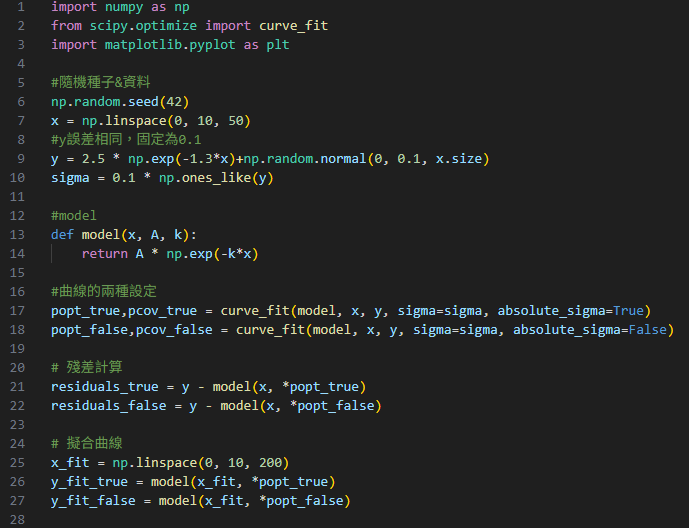
\includegraphics[width=1\linewidth]{1.png}
    \caption{程式碼(1)}
    \label{fig:py1}
\end{figure}

\clearpage

\begin{figure}[h]
    \centering
    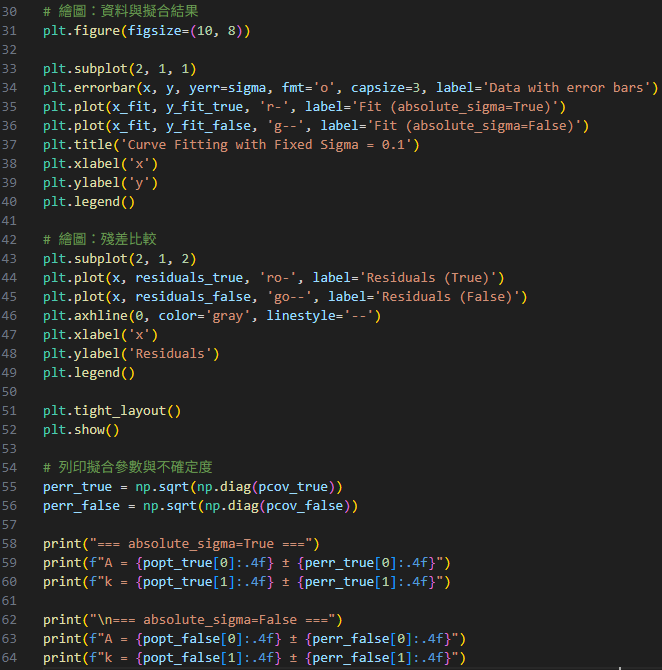
\includegraphics[width=1\linewidth]{2.png}
    \caption{程式碼(2)}
    \label{fig:py2}
\end{figure}

\begin{enumerate}
    \item 設定講義之參數、建立給定模型。
    \item 透過\texttt{curve\_fit}擬合。
    \item 繪出擬合曲線及殘差圖。
    
\end{enumerate}

\clearpage

\section{實驗數據與分析}
\hfill

\begin{figure}[h]
    \centering
    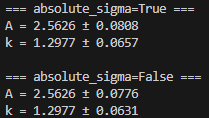
\includegraphics[width=0.5\linewidth]{output3.png}
    \caption{最佳擬合參數}
    \label{fig:op3}
\end{figure}

輸出:

\texttt{absolute\_sigma=True}
\begin{itemize}
    \item $A=2.5626 \pm 0.0808$
    \item $k=1.2977 \pm 0.0657$
\end{itemize}

\texttt{absolute\_sigma=False}
\begin{itemize}
    \item $A=2.5626 \pm 0.0776$
    \item $k=1.2977 \pm 0.0631$
\end{itemize}

\begin{figure}[h]
    \centering
    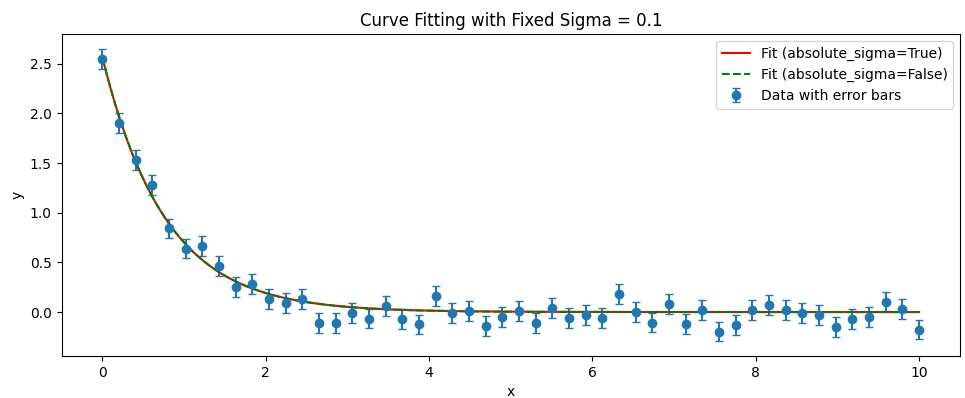
\includegraphics[width=1\linewidth]{output1.png}
    \caption{original data with error bars}
    \label{fig:op1}
\end{figure}

透過Fig.\ref{fig:op1}可以確認擬合出的曲線是否貼近資料點。

同時也可看出,\texttt{absolute\_sigma=True}與\texttt{absolute\_sigma=False}的曲線高度重疊,這是因為 \texttt{absolute\_sigma} 並不會影響擬合曲線,而只會影響參數的誤差估計。

\clearpage

\begin{figure}[h]
    \centering
    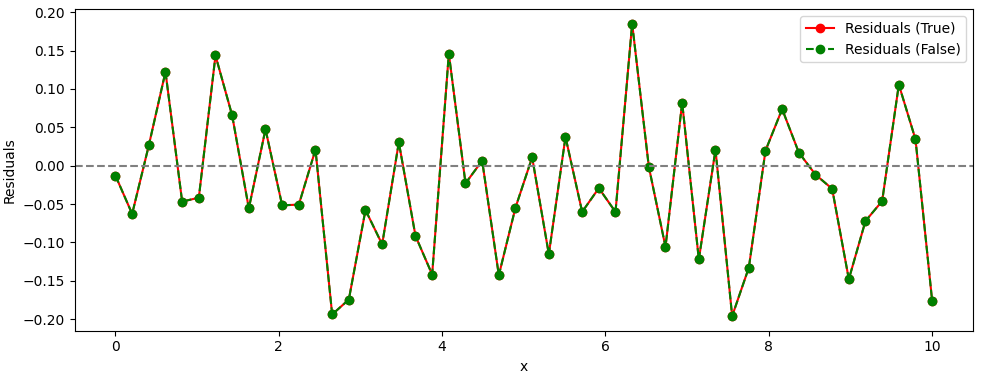
\includegraphics[width=1\linewidth]{output2.png}
    \caption{residuals for each of the two cases separately}
    \label{fig:op-2}
\end{figure}

殘差圖可以比較這兩種擬合之下資料與模型之間的偏差。
可以看出二者的殘差分布皆沒有明顯趨勢,且分布於0附近,顯示出模型與資料吻合程度相當高,可以應證\texttt{absolute\_sigma} 只會影響參數的誤差估計而不影響擬合結果與殘差本身。

\section{問題討論}

\subsection{First, average the five period measurements for each pendulum length and obtain the error bar (standard deviation), then perform the fitting.}
\hfill

回顧上週內容,我們所做的$\chi ^2$ fitting的程式碼(如下Fig.\ref{fig:chi1}到Fig.\ref{fig:chi5})

\begin{figure}[h]
    \centering
    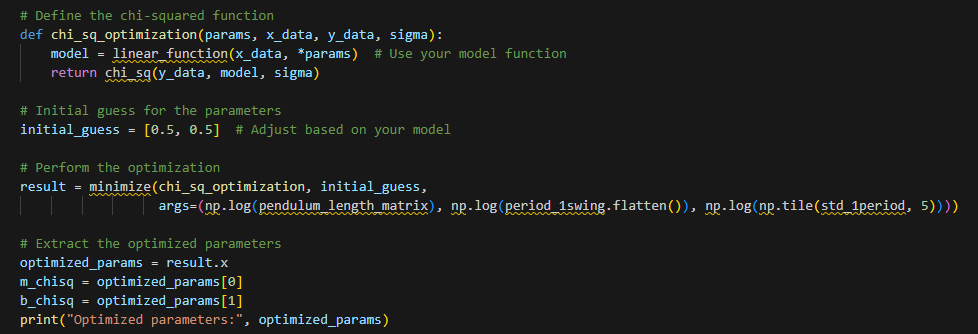
\includegraphics[width=1\linewidth]{chi1.png}
    \caption{$\chi ^2$ fitting程式碼(1)}
    \label{fig:chi1}
\end{figure}

\clearpage

\begin{figure}[h]
    \centering
    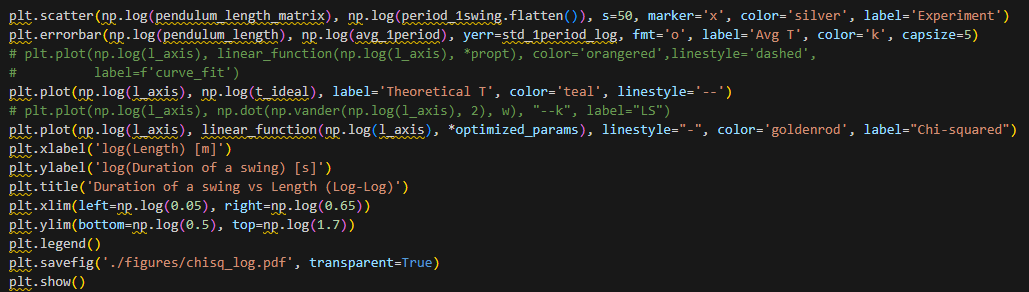
\includegraphics[width=1\linewidth]{chi2.png}
    \caption{$\chi ^2$ fitting程式碼(2)}
    \label{fig:chi2}
\end{figure}


Fig.\ref{fig:chi1}是先定義$\chi ^2$ function,並定義:
\begin{itemize}
    \item params為我們要最佳化的參數(直線之斜率或截距)
    \item $x\_data$和$y\_data$ 為輸入數據
    \item sigma為測量不確定性
    \item linear\_function($x\_data$, \*params) 為一條直線($y=ax+b$)
    \item chi\_sq(y\_data, model, sigma) 為計算$\chi^2$
\end{itemize}


接著設定初始參數,先猜測m=0.5、b=0.5;並進行最小化$\chi^2$。

而因為實驗要求擬合擺動週期與擺長的對數關係,所以需取對數,使其變線性關係(詳情見預習問題1、2)即可求得a、b。最後把最佳化後的m、b,和$\chi^2$值顯示出來。

最終輸出結果:
\begin{itemize}
    \item Optimized parameters: [0.48023142 0.79271392]
    \item Chi-square value: 0.15251356436613928
    \item $reduced \ \chi^2 \approx 0.0019$
\end{itemize}



\begin{figure}[h]
    \centering
    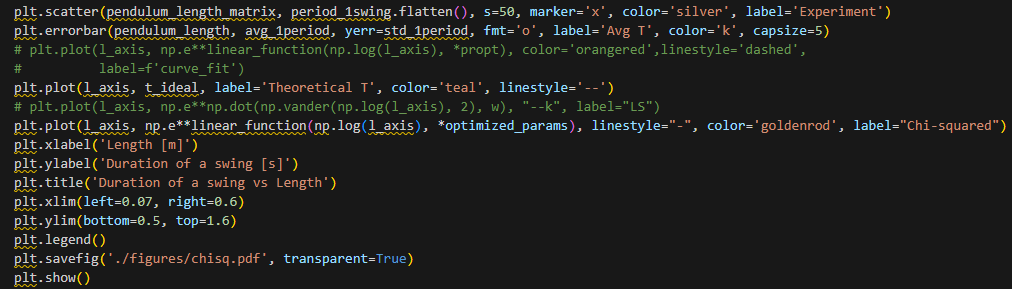
\includegraphics[width=1\linewidth]{chi3.png}
    \caption{$\chi ^2$ fitting程式碼(3)}
    \label{fig:chi3}
\end{figure}


Fig.\ref{fig:chi3}使用\texttt{plt.scatter()}繪製實驗數據點;x軸為擺長取對數;y軸為單次擺動週期取對數。利用交叉符號點出個別數據點。

\clearpage
接著繪出理論曲線和$\chi^2$擬合的曲線,並設定座標軸與標題及範圍;結果為Fig.\ref{fig:chi_sq}右圖。

\begin{figure}[h]
    \centering
    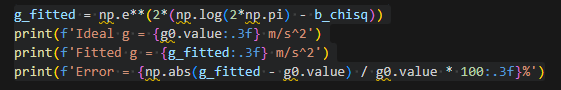
\includegraphics[width=1\linewidth]{chi4.png}
    \caption{$\chi ^2$ fitting程式碼(4)}
    \label{fig:chi4}
\end{figure}

\indent Fig.\ref{fig:chi4}繪製擺長與擺動週期的關係圖,但和上部分的對數-對數圖不同,這次是線性尺度。\\
\indent 令x軸為擺長、y軸為擺動週期,用銀色交叉符號標出實驗數據,並繪出error bar(使用黑色圓點,表測量之不確定性);最後劃出理論曲線和$\chi^2$理論曲線與我們擬合出的結果(Fig.\ref{fig:chi_sq}左圖)。

\begin{figure}[h]
    \centering
    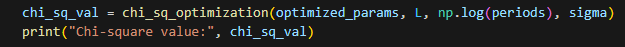
\includegraphics[width=1\linewidth]{chi5.png}
    \caption{$\chi ^2$ fitting程式碼(5)}
    \label{fig:chi5}
\end{figure}
Fig.\ref{fig:chi5}透過$\chi^2$擬合的結果估算重力加速度$g$,並和理論值($g_0$)比較。\\



結果輸出為:
\begin{figure}[h]
    \centering
    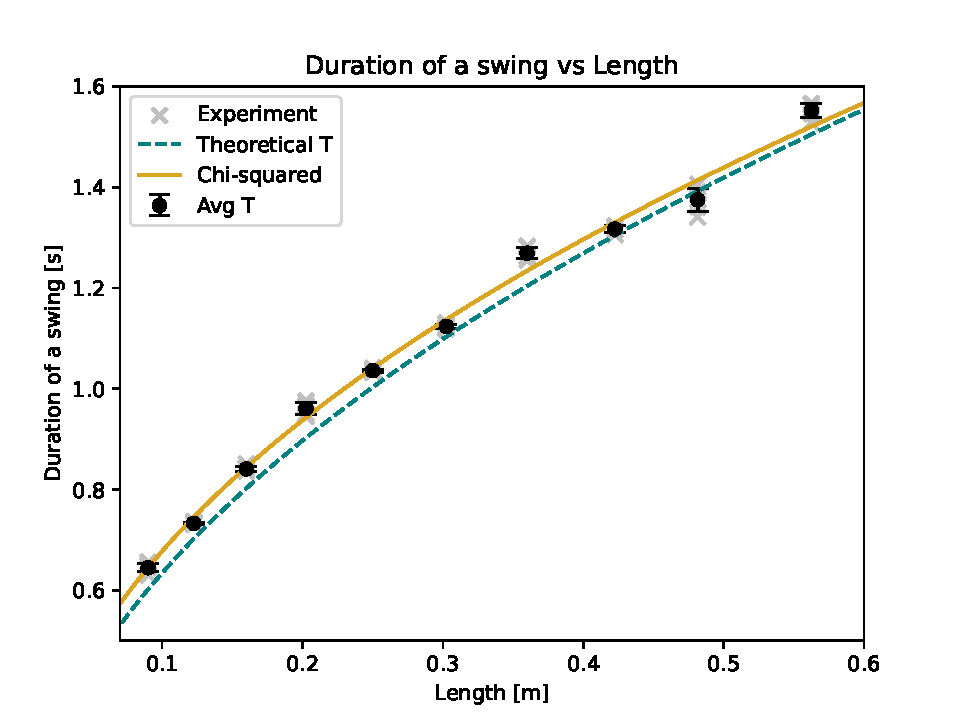
\includegraphics[width=0.49\linewidth]{chisq.pdf}
    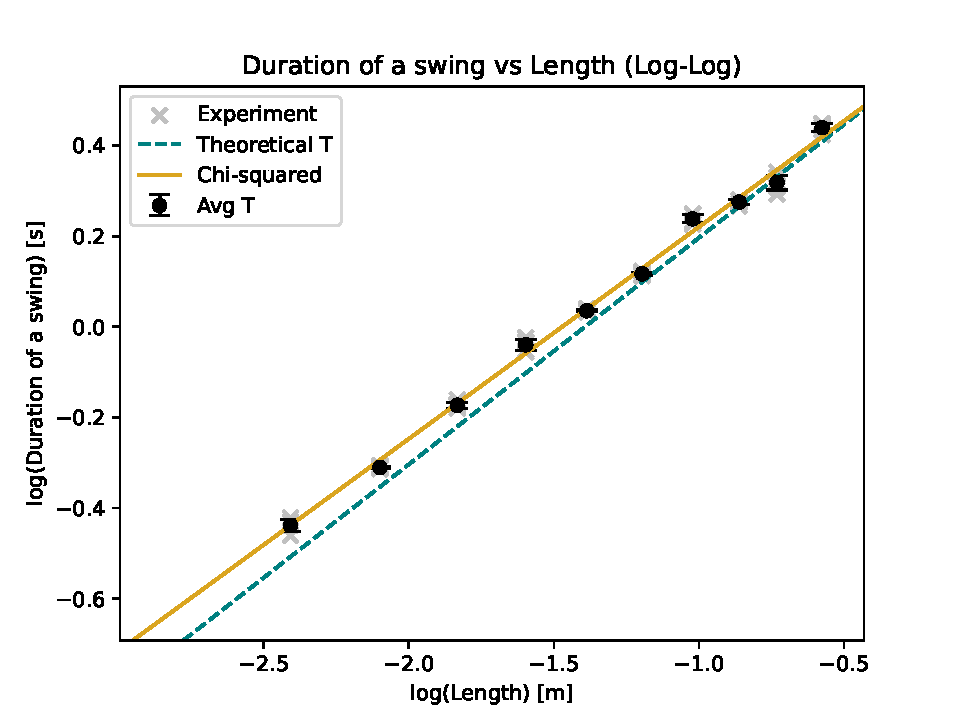
\includegraphics[width=0.49\linewidth]{chisq_log.pdf}
    \caption{數據平均後$\chi^2$擬合結果(左圖為線性擬合;右圖為對數擬合)}
    \label{fig:chi_sq}
\end{figure}

\clearpage

\begin{figure}[h]
    \centering
    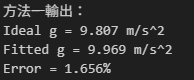
\includegraphics[width=0.5\linewidth]{Q1-1.png}
    \caption{使用數據平均後擬合推測之重力加速度}
    \label{fig:Q1-1}
\end{figure}


殘差圖如下:

\begin{figure}[h]
    \centering
    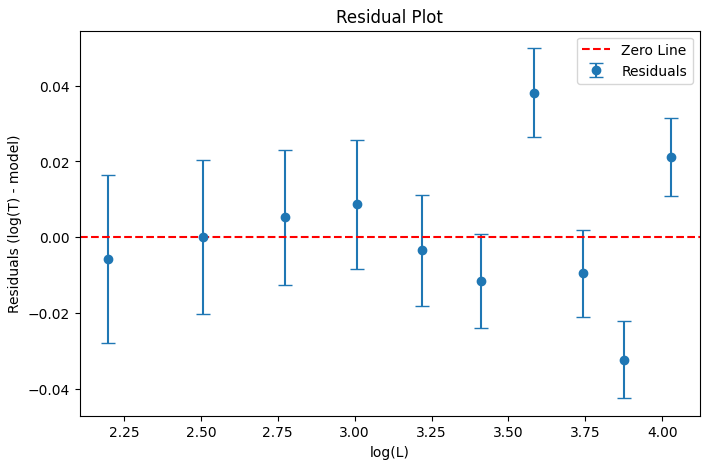
\includegraphics[width=0.8\linewidth]{aaaaaaaaaaaaaaaa.png}
    \caption{數據平均後擬合之殘差圖}
    \label{fig:enter-label}
\end{figure}

\clearpage
\subsection{Fit all 25 data points using the errors obtained by the method mentioned above for $\chi ^2$ fitting.}
\hfill

我們藉由第一題的基礎下再加上以下的程式碼(見Fig.\ref{fig:Q2-1})
\begin{figure}[h]
    \centering
    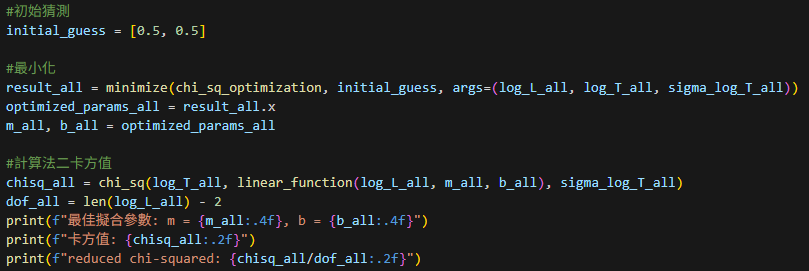
\includegraphics[width=1\linewidth]{Q2.png}
    \caption{將25個數據點做擬合-程式碼(1)}
    \label{fig:Q2-1}
\end{figure}

得到輸出如下:
\begin{itemize}
    \item 最佳擬合參數:$m = 0.4631, b = 0.6802$
    \item 卡方值: 1890.42
    \item reduced $\chi ^2$: 39.38
\end{itemize}


將結果會製成圖:
\begin{figure}[h]
    \centering
    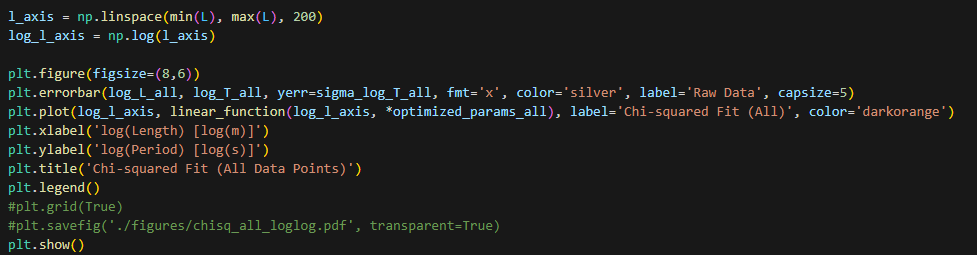
\includegraphics[width=1\linewidth]{Q2-2.png}
    \caption{將25個數據點做擬合-程式碼(2)}
    \label{fig:Q2-2}
\end{figure}

使用對數模型繪出對數-對數圖,輸出見Fig.\ref{fig:chi-all}右圖。

\clearpage

\begin{figure}[h]
    \centering
    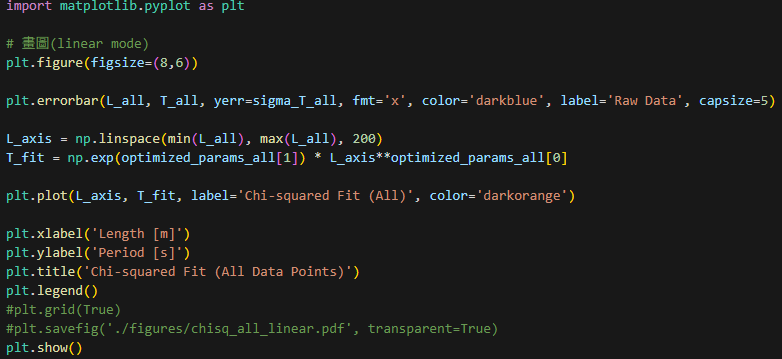
\includegraphics[width=1\linewidth]{Q2-3.png}
    \caption{將25個數據點做擬合-程式碼(3)}
    \label{fig:Q2-3}
\end{figure}

使用線性模型繪出成圖,輸出見Fig.\ref{fig:chi-all}左圖。

\begin{figure}[h]
    \centering
    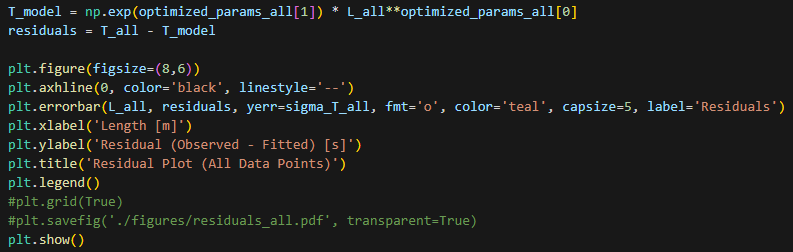
\includegraphics[width=1\linewidth]{Q2-6.png}
    \caption{將25個數據點做擬合-程式碼(4)}
    \label{fig:Q2-6}
\end{figure}


繪出25個數據點的殘差圖,輸出見Fig.\ref{fig:Q2-8}

\clearpage

結果為:
\begin{figure}[h]
    \centering
    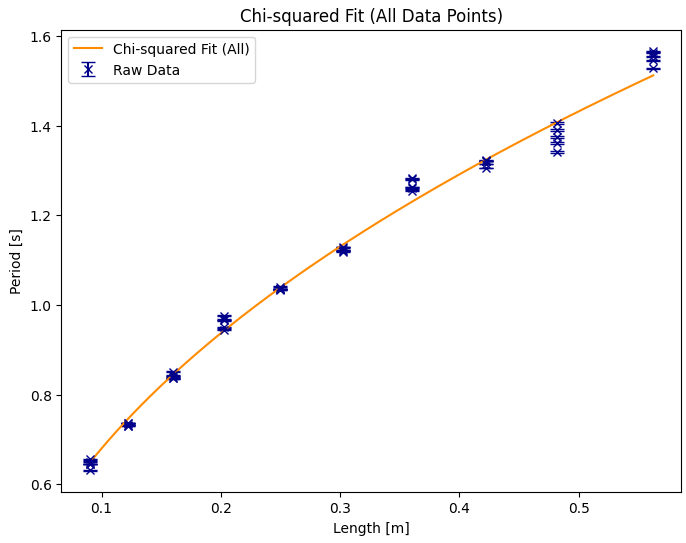
\includegraphics[width=0.45\linewidth]{Q2-op.png}
    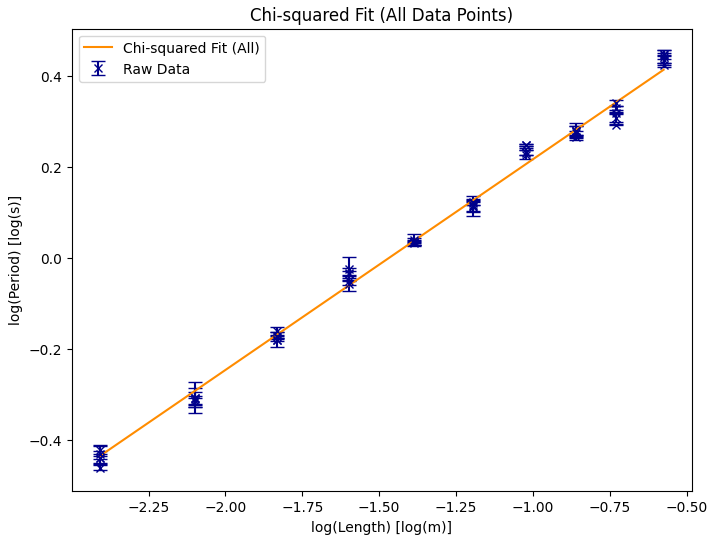
\includegraphics[width=0.45\linewidth]{Q2-op-log.png}
    \caption{25個數據$\chi^2$擬合結果(左圖為線性擬合;右圖為對數擬合)}
    \label{fig:chi-all}
\end{figure}

\begin{figure}[h]
    \centering
    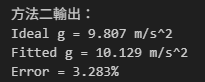
\includegraphics[width=0.45\linewidth]{Q2-4.png}
    \caption{使用25個數據點擬合後推測之重力加速度}
    \label{fig:Q2-4}
\end{figure}

%\clearpage
殘差圖如下:

\begin{figure}[h]
    \centering
    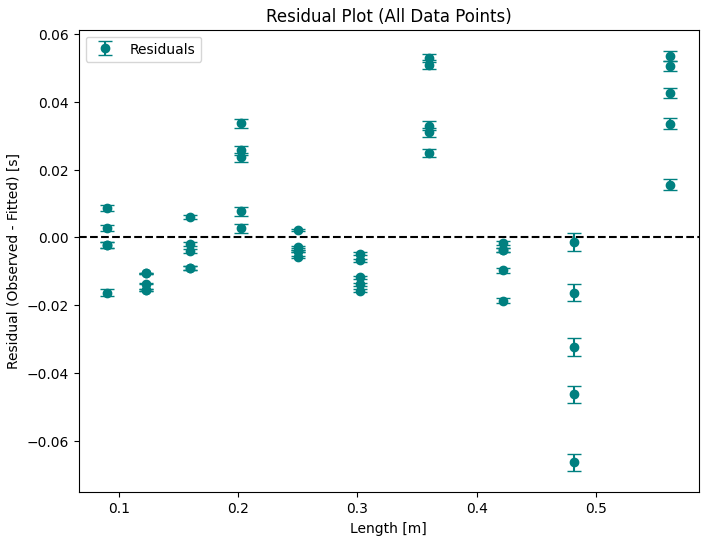
\includegraphics[height=0.3\linewidth]{Q2-8.png}
    \caption{25個數據之殘差圖}
    \label{fig:Q2-8}
\end{figure}

\clearpage

\subsection{分析問題一、二之差距}
\hfill

比較「平均後擬合」與「直接用25筆資料擬合」的結果,可以發現「直接用25筆資料擬合」所得到的 reduced $\chi^2$ 明顯較大,且透過斜率推算出的重力加速度與理論值之誤差也更大,其原因在於每筆原始資料本身皆有測量誤差,且殘差分布較為分散,造成擬合品質下降。

相較之下,「平均後擬合」藉由對每組資料取平均,有效降低了隨機誤差,使擬合結果更為穩定且接近理論預期;而「直接用25筆資料擬合」雖然資料量較多,但誤差的累積與異常值的影響使得擬合結果偏離理論。

%%%%%%%%%%%%%%%%%%%%%%%%%%%%%%%%%%%%%%%%%%%%%%%%%%%%%%%%%%%%

%\subsection{Difference between \texttt{absolute\_sigma=True} and \texttt{=False}}
%或許不一定要寫





\section{總結}
\hfill

本次實驗中,第一部分使用\texttt{scipy.optimize.curve\_fit}函數擬合指數衰減模型,並分別設定\texttt{absolute\_sigma=True}和\texttt{absolute\_sigma=False}兩種情況來比較。

結果顯示兩種設定下擬合曲線高度重疊,代表\texttt{absolute\_sigma}的設定不會影響擬合曲線本身,而是影響參數誤差的估計範圍。

從殘差圖可觀察出,兩種情況的殘差均無明顯的系統性偏差,且皆分布於0附近,表示擬合品質佳。本次模型物理上描述了一個指數衰減的過程,符合資料特性,而主要誤差來源為每個資料點的高斯隨機誤差與統計波動。由於本次實驗中每筆資料的誤差設定一致,且權重相同,因此不論\texttt{absolute\_sigma}設定為True或False,最佳擬合參數(如A和k)幾乎一致,進而導致擬合曲線相同。差異僅體現在擬合後參數誤差(即$\pm$數值)的計算方式上。

關於\texttt{absolute\_sigma}的影響,整理如下:
\begin{itemize}
    \item \texttt{absolute\_sigma=False}(預設值):\\假設資料誤差可能存在低估或高估的情況,\texttt{curve\_fit} 會根據殘差自動調整誤差大小,再以此計算參數的不確定性。
    \item \texttt{absolute\_sigma=True}:\\假設提供的error bars已準確反映真實誤差,因此擬合時不進行額外調整,直接使用輸入的誤差計算參數不確定性。
\end{itemize}

而第二部分的延伸實驗則有兩種$\chi^{2}$擬合結果比較:平均資料後再擬合以及直接使用單次測量資料擬合。結果發現前者的 reduced $\chi^{2}$ 值更接近理想值,且重力加速度的值也更接近理論值。

此次實驗延續前面實驗,繼續了解與學習誤差處理的方式,並透過了解不同的計算方式,學習分析並找出對於不同類型的實驗數據較適合的計算方式,日後能運用於真實實驗數據的分析。


\section{分工}
\begin{itemize}
    \item 洪瑜: $\chi^2$ fitting、誤差討論及問題討論
    \item 黃巧涵: 數據分析
    \item 洪懌平: 摘要、前言
\end{itemize}

%--------------------------------------------------------------
\end{CJK}
\end{document}